\usepackage{graphicx}
\newpage
\thispagestyle{fancy}
\vspace{\fill}
\subsection{Tela de comando Alimentação}
Esta tela é acessada pelo botão \("\)\textgreater\("\) no menu superior esquerdo da tela de comando de máquina, pelo botão \("\)\textless{}" no menu superior esquerdo da tela comando impressoras ou impressora 1, pelo botão \("\)ALM" em qualquer tela de comando e pelo botão comando da tela ajustes alimentação. A partir desta os botões "comando" e "ajustes" começam a se comportar de maneira contextual de maneira que eles vão levar a tela correspondente a tela selecionada. Caso você já esteja na tela selecionada você será levado a tela anterior.
\vspace*{10pt}

\begin{figure}
    \centering
    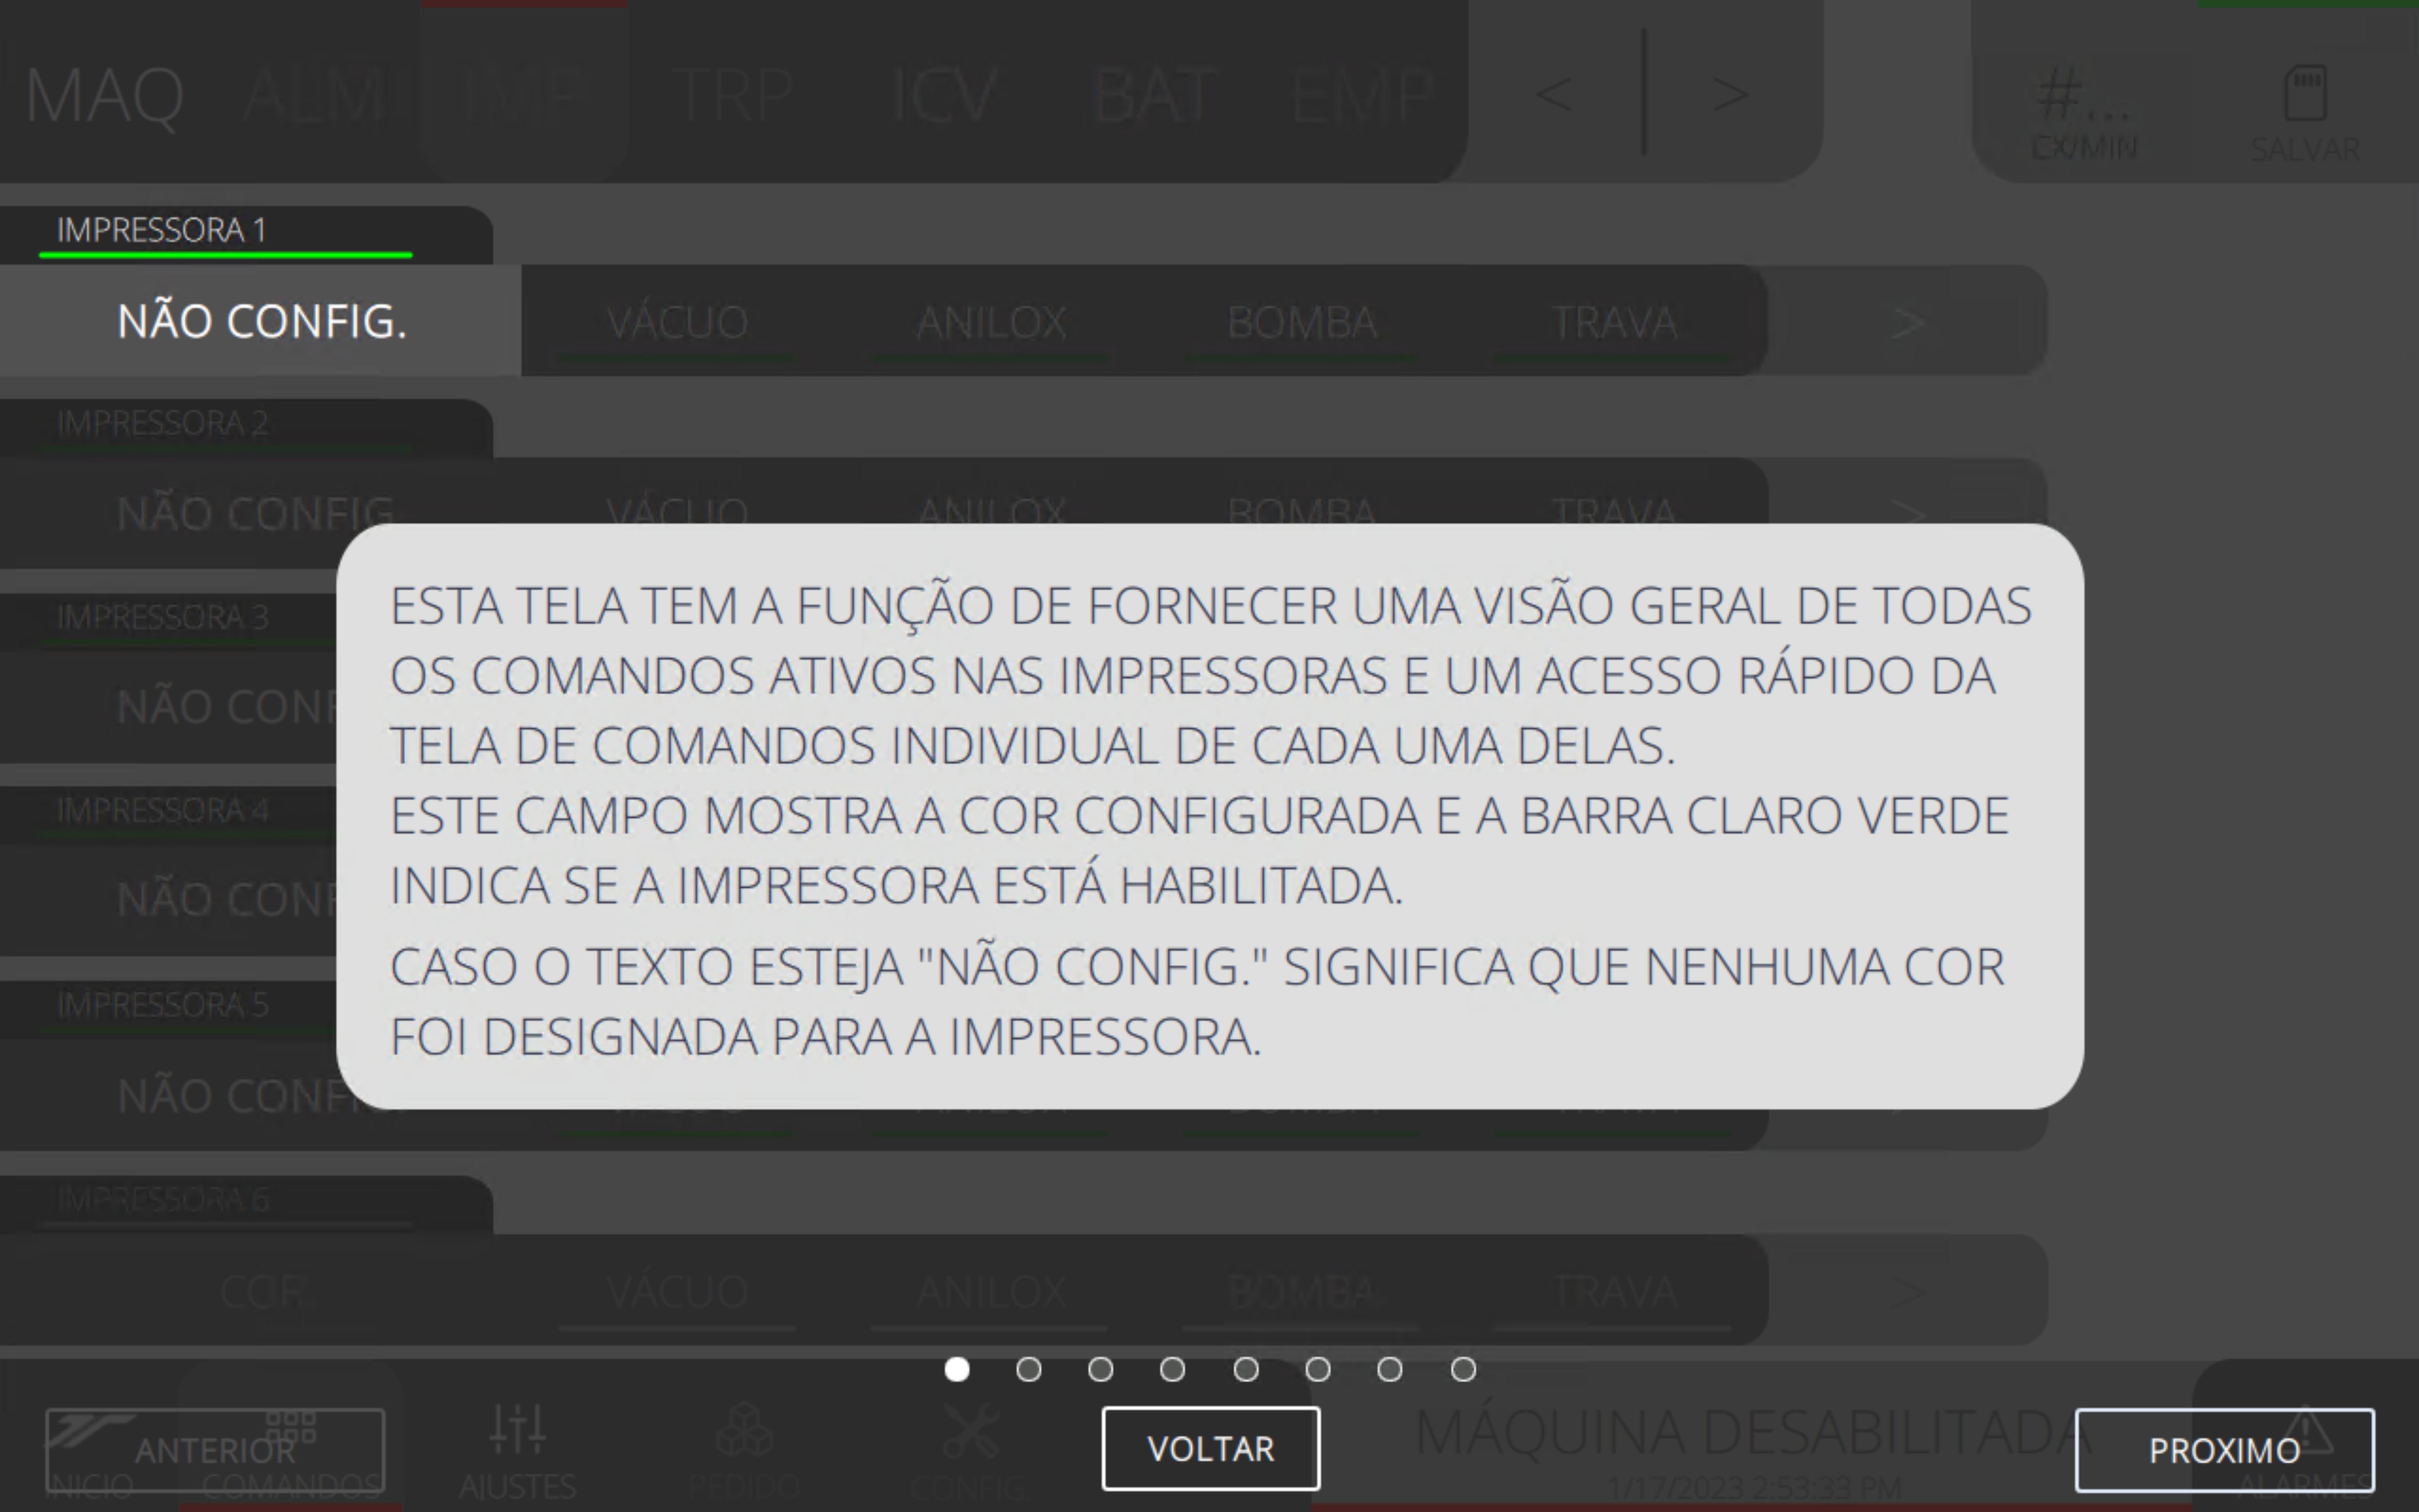
\includegraphics[width=480,height=300]{imagesICV/03-feeder/commands/1}
    \caption{Tela de comando Alimentação}
\end{figure}
\newpage
\thispagestyle{fancy}
\vspace{\fill}

\subsection{Alimentação manual da máquina}

\begin{figure}
    \centering
    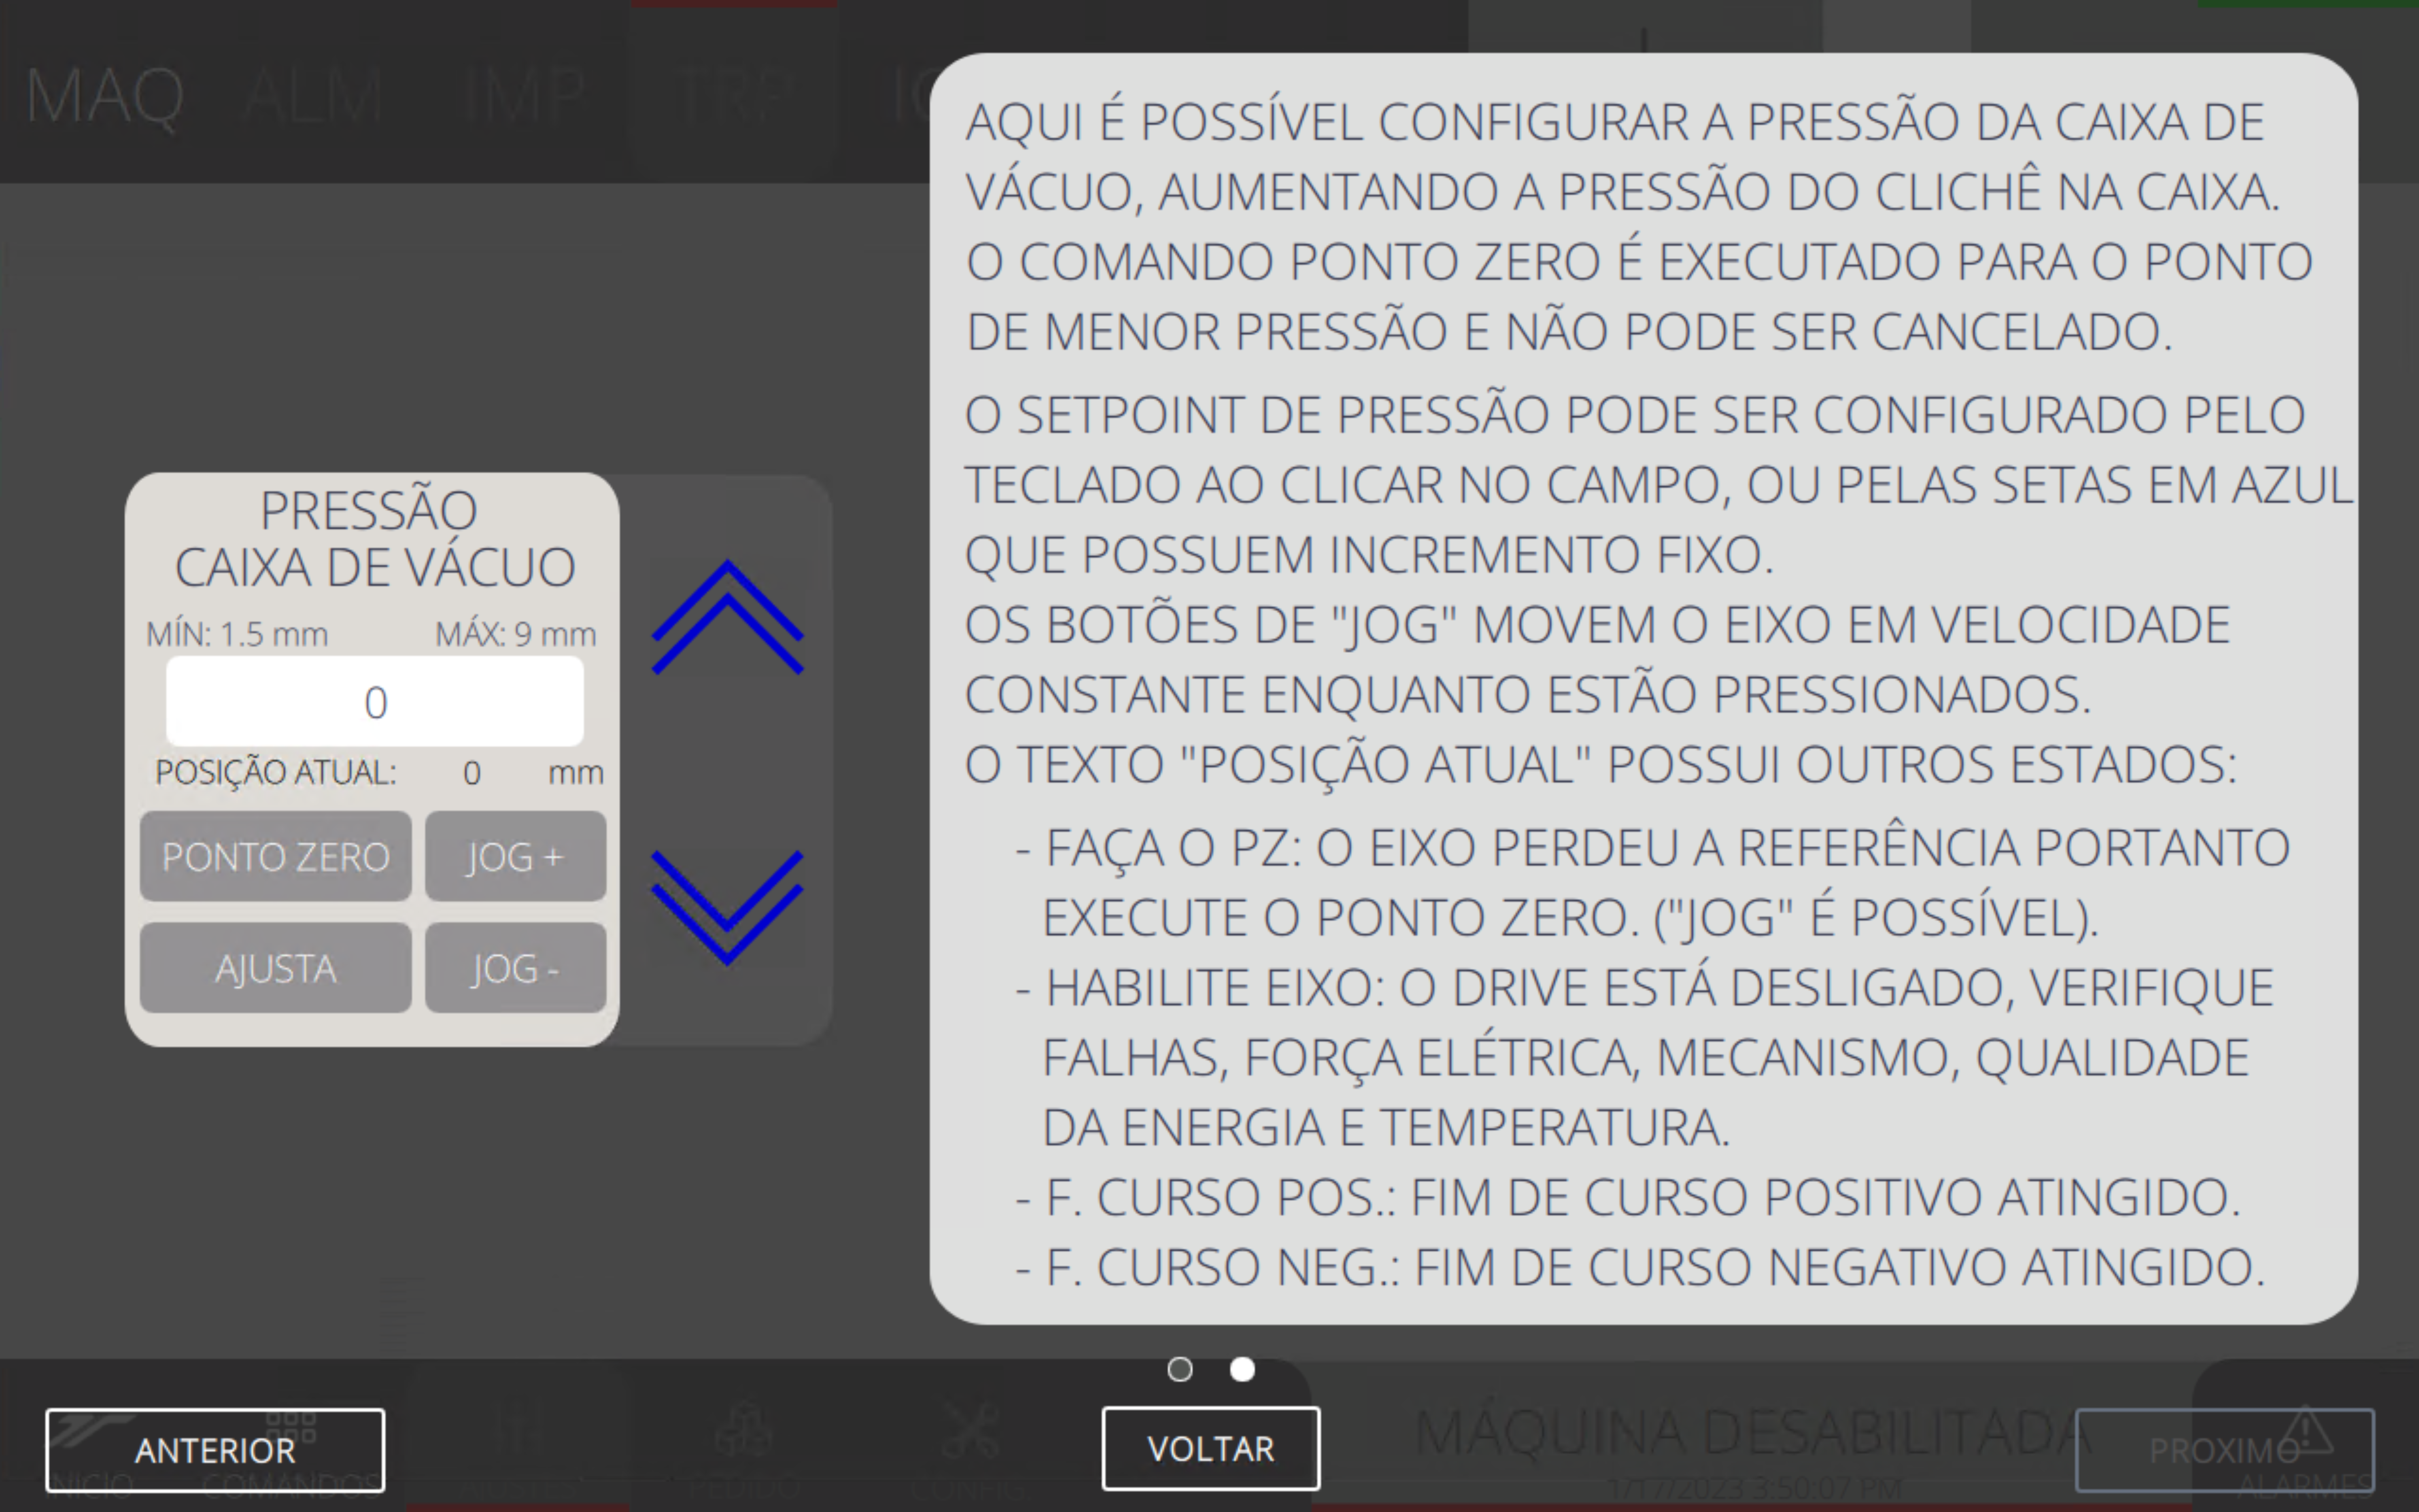
\includegraphics[width=576,height=360]{imagesICV/03-feeder/commands/2}
    \caption{Alimentação manual da máquina}
\end{figure}
\newpage
\thispagestyle{fancy}
\vspace{\fill}

\subsection{Alimentação automática da máquina}
\begin{figure}
    \centering
    \includegraphics[width=576,height=360]{imagesICV/03-feeder/commands/3}
    \caption{Alimentação automática da máquina}
\end{figure}
\newpage
\thispagestyle{fancy}
\vspace{\fill}

\subsection{Habilita vácuo transporte}
\begin{figure}
    \centering
    \includegraphics[width=576,height=360]{imagesICV/03-feeder/commands/4}
    \caption{Habilita vácuo transporte}
\end{figure}
\newpage
\thispagestyle{fancy}
\vspace{\fill}

\subsection{Habilita vácuo alimentação}
\begin{figure}
    \centering
    \includegraphics[width=576,height=360]{imagesICV/03-feeder/commands/5}
    \caption{Habilita vácuo alimentação}
\end{figure}
\newpage
\thispagestyle{fancy}
\vspace{\fill}

\subsection{Executa ponto zero Lançador de Caixas}
\begin{figure}
    \centering
    \includegraphics[width=576,height=360]{imagesICV/03-feeder/commands/6}
    \caption{Executa ponto zero LCX}
\end{figure}
\newpage
\thispagestyle{fancy}
\vspace{\fill}

\subsection{Habilita alimentação de chapas}
\begin{figure}
    \centering
    \includegraphics[width=576,height=360]{imagesICV/03-feeder/commands/7}
    \caption{Habilita alimentação de chapas}
\end{figure}
\newpage
\thispagestyle{fancy}
\vspace{\fill}

\subsection{Trava unidade alimentação}
\begin{figure}
    \centering
    \includegraphics[width=576,height=360]{imagesICV/03-feeder/commands/8}
    \caption{Trava unidade alimentação}
\end{figure}
\newpage
\thispagestyle{fancy}
\vspace{\fill}

\subsection{Habilita barra eletrostática]}
\begin{figure}
    \centering
    \includegraphics[width=576,height=360]{imagesICV/03-feeder/commands/9}
    \caption{Habilita barra eletrostática}
\end{figure}